% Source-SHA256: 0bf7df5e4d89fced17b2f6ee040d07c9590aeb053e93ab050c1fdf252fdd402c
% !TeX program = xelatex
\documentclass[a4paper,11pt]{article}
\usepackage{fontspec}
\IfFontExistsTF{TeX Gyre Pagella}{\setmainfont{TeX Gyre Pagella}}{\setmainfont{P052}}
\IfFontExistsTF{TeX Gyre Heros}{\setsansfont{TeX Gyre Heros}}{\setsansfont{Nimbus Sans}}
\IfFontExistsTF{TeX Gyre Cursor}{\setmonofont{TeX Gyre Cursor}[Scale=0.88]}{\setmonofont{Nimbus Mono PS}[Scale=0.88]}
\usepackage{babel}
\babelprovide[import,main]{spanish}
\usepackage{microtype}
\usepackage[a4paper,margin=2.4cm,headheight=23pt,headsep=10pt,footskip=1.1cm]{geometry}
\raggedbottom
\setlength{\emergencystretch}{3em}
\hyphenpenalty=10000
\exhyphenpenalty=10000
\clubpenalty=10000
\widowpenalty=10000
\usepackage{xcolor}
\definecolor{navybg}{HTML}{0B1D2E}
\definecolor{navydeep}{HTML}{123049}
\definecolor{lightblue}{HTML}{8FD3FE}
\definecolor{amber}{HTML}{F5A623}
\definecolor{softgray}{HTML}{5B6570}
\usepackage{titlesec,needspace}
\setcounter{secnumdepth}{-1}
\setcounter{tocdepth}{2}
\titleformat{\section}{\sffamily\Large\bfseries\color{navydeep}\raggedright}{}{0pt}{}
\titleformat{\subsection}{\sffamily\large\bfseries\color{navydeep}\raggedright}{}{0pt}{}
\titlespacing*{\section}{0pt}{20pt}{9pt}
\titlespacing*{\subsection}{0pt}{14pt}{6pt}
\usepackage{fancyhdr}
\pagestyle{fancy}
\fancyhf{}
\fancyhead[L]{\small\sffamily\color{softgray}Compás a compás}
\fancyhead[R]{\small\sffamily\color{softgray}Diseño técnico del software}
\fancyfoot[L]{\small\sffamily\color{softgray}Aplicación 0.7.3 · 26/10/2026}
\fancyfoot[R]{\small\sffamily\color{softgray}\thepage}
\renewcommand{\headrulewidth}{0.4pt}
\usepackage{array,longtable,booktabs,calc}
\newcounter{none}
\renewcommand{\arraystretch}{1.15}
\usepackage{enumitem}
\setlist[itemize]{leftmargin=1.4em,itemsep=3pt,topsep=5pt}
\setlist[enumerate]{leftmargin=1.8em,itemsep=3pt,topsep=5pt}
\usepackage{fvextra,framed,seqsplit}
\fvset{fontsize=\small,breaklines=true,breakanywhere=true,frame=leftline,framerule=1.4pt,rulecolor=\color{lightblue},framesep=8pt}
\RecustomVerbatimEnvironment{verbatim}{Verbatim}{breaklines,breakanywhere,samepage=true,fontsize=\small}
\let\originaltexttt\texttt
\renewcommand{\texttt}[1]{\originaltexttt{\seqsplit{#1}}}
\providecommand{\tightlist}{\setlength{\itemsep}{2pt}\setlength{\parskip}{0pt}}
% Pandoc 3.2+ envuelve las imágenes en \pandocbounded; con versiones anteriores no existe y esta definición no cambia nada.
\providecommand{\pandocbounded}[1]{#1}
\usepackage{graphicx,xurl,tikz}
\usepackage[section]{placeins}
\usepackage{amssymb,newunicodechar}
\usepackage[colorlinks=true,linkcolor=navydeep,urlcolor=navydeep,pdftitle={Compás a compás - Diseño técnico del software},pdfauthor={Jesús Quevedo Rodríguez}]{hyperref}
\usepackage{bookmark}
\newunicodechar{♭}{\texorpdfstring{\ensuremath{\flat}}{\unichar{9837}}}
\newunicodechar{♯}{\texorpdfstring{\ensuremath{\sharp}}{\unichar{9839}}}
\newunicodechar{✓}{\texorpdfstring{\ensuremath{\checkmark}}{\unichar{10003}}}
\newunicodechar{✗}{\texorpdfstring{\ensuremath{\times}}{\unichar{10007}}}
\newunicodechar{→}{\texorpdfstring{\ensuremath{\rightarrow}}{\unichar{8594}}}
\newunicodechar{←}{\texorpdfstring{\ensuremath{\leftarrow}}{\unichar{8592}}}
\setlength{\parindent}{0pt}
\setlength{\parskip}{6pt}
\renewcommand{\topfraction}{0.95}
\renewcommand{\bottomfraction}{0.95}
\renewcommand{\textfraction}{0.05}
\renewcommand{\floatpagefraction}{0.6}
\setcounter{topnumber}{3}
\setcounter{totalnumber}{4}
\begin{document}
\begin{titlepage}
\newgeometry{margin=0cm}
\thispagestyle{empty}
\pagecolor{navybg}
\color{white}
\vspace*{3cm}
\begin{center}
{\sffamily\bfseries\fontsize{16}{19}\selectfont\color{amber} COMPÁS A COMPÁS\par}
\vspace{1cm}
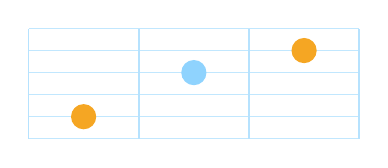
\begin{tikzpicture}[x=0.7cm,y=0.28cm]
\foreach \y in {0,...,5} {\draw[lightblue!55,line width=0.5pt] (-3,\y)--(3,\y);}
\foreach \x in {-3,-1,1,3} {\draw[lightblue!65,line width=0.6pt] (\x,0)--(\x,5);}
\fill[amber] (-2,1) circle[x radius=0.16cm,y radius=0.16cm];
\fill[lightblue] (0,3) circle[x radius=0.16cm,y radius=0.16cm];
\fill[amber] (2,4) circle[x radius=0.16cm,y radius=0.16cm];
\end{tikzpicture}\par
\vspace{1.4cm}
{\sffamily\bfseries\fontsize{30}{38}\selectfont Diseño técnico del software\par}
\vspace{0.8cm}
{\sffamily\fontsize{14}{20}\selectfont\color{lightblue} Arquitectura, datos, paginación y operación local\par}
\vfill
{\sffamily\small Autor del proyecto: Jesús Quevedo Rodríguez\par}
{\sffamily\small Aplicación 0.7.3 · 26/10/2026\par}
{\sffamily\small Repositorio: a01653/Compas-a-compas\par}
\vspace{2cm}
\end{center}
\end{titlepage}
\nopagecolor
\restoregeometry
\setcounter{page}{2}
\tableofcontents
\newpage
Aplicación 0.7.3 · Esquema de canción 1 · Edición del DTS: 26/10/2026.
Autor del proyecto: Jesús Quevedo Rodríguez.

\Needspace{3.5cm}
\section{Objeto y alcance}\label{objeto-y-alcance}

Compás a compás es un editor local de hojas de acordes de guitarra.
Organiza una canción en compases, admite varios acordes por compás y
varias digitaciones por acorde. Genera una vista previa paginada y una
salida HTML autónoma para impresión A4 horizontal.

Este documento describe la versión 0.6.0, con interfaz compacta, textos
sin bloques duplicados, historial de acciones, marcas por compás, paleta
editable y tonalidades por posición. Incluye el lanzador de Windows. Los
requisitos originales permanecen en \texttt{docs/REQUISITOS.md}; el
historial de implementación y sus comprobaciones está en
\texttt{docs/ESTADO.md}. Este DTS describe el comportamiento vigente,
por encima de las medidas históricas de fases anteriores.

No se incluyen reproducción, OCR, transposición, análisis armónico,
generación automática de posiciones ni sincronización en la nube. Las
marcas musicales son notación escrita: no hay un motor que ejecute o
expanda el recorrido.

\Needspace{3.5cm}
\section{Arquitectura y ejecución}\label{arquitectura-y-ejecuciuxf3n}

\subsection{Componentes}\label{componentes}

La aplicación usa HTML, CSS y módulos JavaScript nativos. No tiene
framework, backend de negocio, base de datos ni dependencias npm de
ejecución. Node.js 18 o superior sirve los archivos al navegador
mediante HTTP local.

{\def\LTcaptype{none} % do not increment counter
\begin{longtable}[]{@{}>{\raggedright\arraybackslash}p{\dimexpr0.333333\linewidth-1.333333\tabcolsep\relax}>{\raggedright\arraybackslash}p{\dimexpr0.333333\linewidth-1.333333\tabcolsep\relax}>{\raggedright\arraybackslash}p{\dimexpr0.333333\linewidth-1.333333\tabcolsep\relax}@{}}
\toprule\noalign{}
Capa & Archivos principales & Responsabilidad \\
\midrule\noalign{}
\endhead
\bottomrule\noalign{}
\endlastfoot
Entrada y estado & \texttt{src/main.js}, \texttt{src/store.js} &
Inicialización, canción única, selección y notificaciones de cambio \\
Modelo & \texttt{src/model/} & Entidades, IDs, validación,
serialización, listas y referencias musicales \\
Geometría & \texttt{src/geometry/fretboard.js} & Intervalo visible y
coordenadas del mástil \\
Renderizado & \texttt{src/render/} & Tarjetas, cabeceras, compases y
marcas mediante DOM y SVG \\
Paginación & \texttt{src/layout/} & Fuentes, unidades, medición DOM y
reparto en filas y hojas \\
Interfaz & \texttt{src/ui/} & Edición, archivos, diálogos, zoom, vista
previa y exportación \\
Recuperación & \texttt{src/persist/recovery.js} & Copia local de cambios
pendientes \\
Salida & \texttt{src/export/document.js} & Ensamblado del HTML
autónomo \\
Arranque & \texttt{Abrir-Compas.cmd}, \texttt{scripts/launch.mjs},
\texttt{scripts/serve.mjs} & Lanzador y servidor estático local \\
\end{longtable}
}

Los estilos de interfaz están en \texttt{styles/app.css}; la hoja usa
estilos compartidos de \texttt{styles/sheet.css}, tokens y exportación.
Las fuentes Caveat Brush y Gochi Hand están incluidas en
\texttt{references/fonts.css}, sin descarga de fuentes remotas. El icono
de la aplicación es \texttt{assets/icon.svg}.

\subsection{Flujo de datos}\label{flujo-de-datos}

\begin{enumerate}
\def\labelenumi{\arabic{enumi}.}
\tightlist
\item
  El usuario modifica la canción mediante un controlador de interfaz.
\item
  El controlador notifica el tipo de cambio al almacén.
\item
  Los paneles afectados actualizan su presentación.
\item
  Si cambió el contenido, el paginador obtiene una copia de la canción,
  carga las fuentes y mide el mismo renderizador que se usará en la
  salida.
\item
  El reparto puro decide filas, fragmentos y páginas; la vista previa
  muestra el último resultado vigente.
\item
  Exportar espera ese resultado, comprueba que sigue vigente y construye
  el HTML desde su copia medida.
\end{enumerate}

El JSON conserva el contenido editable. Coordenadas, filas, número de
páginas y zoom son datos derivados y no se guardan como parte de la
canción.

\Needspace{3.5cm}
\section{Interfaz compacta y contexto de
compás}\label{interfaz-compacta-y-contexto-de-compuxe1s}

El editor usa dos columnas: controles de compás y tarjeta a la
izquierda, y hoja a la derecha. Los selectores permiten recorrer listas
extensas sin aumentar la altura del formulario. Digitación, grados y
textos están siempre visibles en dos secciones apiladas, sin controles
de pestaña. Nombre, tonalidad y versión del documento se editan en un
diálogo. Exportar agrupa HTML e impresión. Los iconos tienen nombre
accesible y los menús se cierran con Escape o al pulsar fuera.

El acceso a Marcas pertenece al bloque Compás y anuncia su etiqueta en
el nombre accesible. El panel filtra símbolos y saltos por el compás
donde están escritos, y repeticiones y casillas por todos los compases
del tramo, incluidos sus extremos. \texttt{src/model/marksContext.js}
obtiene esa vista sin modificar la estructura. Un extremo desaparecido
sigue siendo localizable desde el que existe; todas las marcas
permanecen accesibles en la vista global.

Cambiar de compás reinicia el borrador del formulario con ese compás
como punto de partida y termina la edición local no guardada; no cambia
marcas persistidas. Elegir otra tarjeta dentro del mismo compás conserva
el borrador. Las marcas existentes se editan usando sus IDs y sus
destinos originales, aunque el tramo empiece en otro compás. Ver todas
las marcas cambia solo el filtro; los avisos globales continúan visibles
en ambas vistas.

\texttt{ui/workspace.js} coordina los diálogos y el contador, y
\texttt{ui/marks.js} gestiona el contexto y el formulario.
\texttt{styles/workspace.css} adapta el espacio a la altura disponible.
El móvil usa paneles apilados; avisos extensos, formularios largos y
varias hojas mantienen desplazamiento cuando se necesita. Las nuevas
cabeceras de tarjeta cambian la composición de la hoja, compartida con
la exportación. La geometría del mástil no cambia.

\Needspace{3.5cm}
\section{Paleta editable}\label{paleta-editable}

\texttt{src/model/palette.js} define la resolución de colores, sus
valores originales y el contraste del texto. El campo opcional
\texttt{song.palette} contiene \texttt{families}, \texttt{degrees} y
\texttt{note}. La paleta se valida con el mismo contrato en el esquema
JSON y el validador manual. Los colores son exclusivamente hexadecimales
de seis cifras; no se aceptan valores CSS arbitrarios. Las etiquetas
personalizadas tienen entre 1 y 32 caracteres y excluyen claves
reservadas de objetos JavaScript.

El esquema 1 se amplía de forma opcional: los archivos anteriores siguen
válidos y se guardan sin cambios si no se personalizan. Un archivo con
\texttt{palette} requiere 0.3.0 o posterior; los lectores anteriores
rechazan el campo desconocido. No se presenta esa compatibilidad como
lectura posible en ambos sentidos.

El panel \texttt{ui/colors.js} ofrece familias, grados naturales y
alterados del 1 al 13, etiquetas personalizadas y notas sin grado. Solo
modifica la paleta de la canción; las notas, IDs, textos y destinos se
conservan. La normalización acepta ♭/♯ como b/\#. Cada etiqueta puede
personalizarse de forma independiente. La restauración individual retira
su entrada; la restauración completa, tras confirmar, elimina
\texttt{palette}.

El contexto de hoja pasa la paleta a tarjetas y mástiles, compartiendo
medición, vista previa y exportación. Los textos y trazos interiores se
adaptan al fondo; los títulos exteriores mantienen su color sobre el
papel. Los colores de notas se serializan en SVG y los fondos como
variables CSS locales. La impresión usa el mismo documento. No se
modifican geometría ni digitaciones al cambiar un color. Las notas al
aire conservan el dibujo de círculo o punto según tengan grado.

\Needspace{3.5cm}
\section{Modelo y contrato JSON}\label{modelo-y-contrato-json}

El contrato formal es \texttt{schemas/song.schema.json}.
\texttt{src/model/validate.js} implementa la validación utilizada por la
aplicación sin cargar una biblioteca externa.
\texttt{src/model/serialize.js} convierte entre objetos y JSON con
sangría de dos espacios y salto final.

\subsection{Entidades}\label{entidades}

{\def\LTcaptype{none} % do not increment counter
\begin{longtable}[]{@{}>{\raggedright\arraybackslash}p{\dimexpr0.320000\linewidth-1.000000\tabcolsep\relax}>{\raggedright\arraybackslash}p{\dimexpr0.680000\linewidth-1.000000\tabcolsep\relax}@{}}
\toprule\noalign{}
Entidad & Contenido \\
\midrule\noalign{}
\endhead
\bottomrule\noalign{}
\endlastfoot
Canción & \texttt{schemaVersion}, \texttt{title}, \texttt{key},
\texttt{measures}, \texttt{structure}; \texttt{documentVersion},
\texttt{keyFamily}, \texttt{showTonalities},
\texttt{showMeasureNumbers}, \texttt{maxMeasuresPerRow},
\texttt{fretboardScalePercent} y \texttt{palette} opcionales; los
compases admiten \texttt{repeatPrevious} y \texttt{repeatPreviousTwo}
(ver DATOS.md) \\
Compás & \texttt{id}, \texttt{label} y lista ordenada
\texttt{chordEvents} \\
Acorde & \texttt{id}, \texttt{chordName}, lista \texttt{voicings};
familia y textos opcionales \\
Posición & \texttt{id}, \texttt{frets} de seis valores; grados, textos,
\texttt{voicingDegree}, \texttt{anchorFret} y \texttt{tonality}
opcionales \\
Estructura & Listas \texttt{repeats}, \texttt{endings}, \texttt{markers}
y \texttt{jumps} \\
\end{longtable}
}

Los trastes se almacenan de sexta a primera cuerda: entero no negativo o
\texttt{null} para una cuerda muda. Los grados, cuando existen, son seis
textos en el mismo orden. \texttt{anchorFret} es un entero positivo
opcional que pinta una columna de referencia más oscura y amplía el
rango del mástil cuando hace falta. La versión de esquema es numérica y
vale 1; la versión de documento es texto libre del usuario. Ninguna de
ellas es la versión del programa.

Ejemplo mínimo válido:

\begin{verbatim}
{
  "schemaVersion": 1,
  "title": "Ejemplo",
  "key": "Do menor",
  "measures": [{
    "id": "m1", "label": "1",
    "chordEvents": [{
      "id": "e1", "chordName": "Cm7",
      "voicings": [{"id": "v1", "frets": [null, 3, 5, 3, 4, 3]}]
    }]
  }],
  "structure": {"repeats": [], "endings": [], "markers": [], "jumps": []}
}
\end{verbatim}

\texttt{examples/cancion-demo.json} amplía el ejemplo con dos posiciones
de un acorde, dos acordes en otro compás, cuatro trastes visibles,
repeticiones, casillas y saltos. Es una demostración, no una
transcripción musical.

\subsection{Tarjetas independientes}\label{tarjetas-independientes}

\texttt{src/model/cards.js} presenta una lista plana sobre los eventos y
posiciones del esquema 1. Abrir, seleccionar y guardar no separa eventos
antiguos. Al cambiar el nombre o familia de una posición compartida,
\texttt{isolateCard} divide el evento conservando orden, IDs de
posiciones y textos efectivos. La primera parte mantiene el ID del
evento original. Añadir o duplicar inserta inmediatamente después de la
tarjeta activa; quitar borra solo esa tarjeta. Las marcas continúan
referidas al compás. El historial conserva las divisiones y sus
selecciones para deshacer y rehacer.

\subsection{Contexto tonal por
tarjeta}\label{contexto-tonal-por-tarjeta}

\texttt{src/model/tonality.js} resuelve el contexto según el orden
escrito. La tonalidad general inicia el recorrido con
\texttt{keyFamily}, o con \texttt{other} si falta. Sin tonalidad general
ni cambio previo no hay contexto. Cada objeto \texttt{voicing.tonality},
con \texttt{text} visible y \texttt{family} válida, establece un cambio;
su ausencia hereda el contexto anterior. El contexto se deriva, no se
serializa por duplicado, y no expande las repeticiones.

\texttt{voicingDegree} es texto manual de la esquina superior derecha,
distinto de los seis \texttt{degrees} de cuerda. Vaciar ese campo o la
tonalidad retira su propiedad. Ambos pertenecen a una tarjeta, como el
título y la anotación. Elegir una calidad con tonalidad vacía es un
borrador del control y no guarda un cambio invisible.

\texttt{showTonalities} es un booleano opcional, visible por defecto.
Oculta las franjas en todas las hojas sin borrar datos y conserva la
tonalidad de cabecera. La casilla y los campos forman parte del
historial y de la recuperación. La familia de la tonalidad usa la paleta
de canción, independientemente de la familia del acorde.

Estos campos amplían el esquema 1 de forma opcional. Los archivos
anteriores siguen válidos sin migración ni modificación silenciosa; un
archivo que incluya campos nuevos necesita 0.5.0 o posterior. Los
validadores manual y JSON Schema rechazan tipos, familias y propiedades
desconocidos.

\subsection{Identidad y validación}\label{identidad-y-validaciuxf3n}

Los identificadores son estables y únicos en el documento. La etiqueta
del compás es independiente de su posición en el array. Mover o
renombrar un compás no cambia sus referencias. Duplicar crea IDs nuevos.
La fábrica reserva también identificadores de referencias pendientes
para evitar que una entidad posterior capture un destino borrado.

La apertura valida antes de sustituir el estado actual. JSON mal
formado, tipos incorrectos, campos desconocidos, IDs duplicados o una
versión de esquema no admitida producen errores y dejan intacta la
canción abierta. No se eliminan silenciosamente campos desconocidos.

La validación distingue la forma del archivo de sus referencias
semánticas. Un destino musical ausente puede conservarse con aviso; no
se reasigna por índice ni por una etiqueta parecida. Al exportar
referencias pendientes se pide confirmación.

\subsection{Textos e importación de
listas}\label{textos-e-importaciuxf3n-de-listas}

El acorde puede definir \texttt{aboveText} e \texttt{insideText}. En una
posición, la ausencia del campo significa heredar; una cadena propia
sustituye el texto y la cadena vacía lo oculta. Se mantiene la
diferencia al guardar y abrir. El formulario 0.6.0 muestra el texto
efectivo y modifica solo la tarjeta seleccionada.
\texttt{setCardTextValue} escribe la excepción individual, incluida la
cadena vacía; si la tarjeta está pendiente, modifica el texto de su
evento. El formato conserva sus valores comunes por compatibilidad, sin
controles de edición compartida en la interfaz.

El importador usa una línea por compás:
\texttt{etiqueta\ \textbar{}\ acorde\ @\ digitación}. Separa eventos por
\texttt{;} y posiciones mediante \texttt{/} tras \texttt{@}. Conserva
nombres como \texttt{C/E}. Genera una previsualización y añade el lote
al final únicamente si todas las líneas son válidas. No calcula
duraciones ni grados.

\Needspace{3.5cm}
\section{Estado, edición y
persistencia}\label{estado-ediciuxf3n-y-persistencia}

\texttt{createStore} mantiene una canción mutable y una selección por
IDs. Guarda además el nombre de archivo, el zoom, la firma del último
guardado y el indicador de cambios pendientes. La firma se obtiene con
\texttt{JSON.stringify}; \texttt{markSaved} actualiza la referencia de
guardado.

Los tipos de cambio son \texttt{text}, \texttt{structure},
\texttt{document}, \texttt{history}, \texttt{selection}, \texttt{zoom} y
\texttt{status}. Un cambio de texto actualiza la hoja sin reconstruir
todos los controles, para conservar el foco. Cambios estructurales o de
documento normalizan la selección a objetos existentes. Selección, zoom
y estado de guardado no provocan una nueva paginación.

Nuevo y Abrir gestionan los cambios pendientes antes de reemplazar el
documento. Guardar usa el selector de archivos cuando el navegador lo
permite y, como alternativa, una descarga con Blob. Cancelaciones y
errores se muestran sin sustituir la canción por un archivo fallido.
Exportar HTML e imprimir no marcan el JSON como guardado.

La recuperación usa la clave \texttt{compas-a-compas:recuperacion:v1} de
\texttt{localStorage}, con fecha de guardado y canción serializada. Se
ofrece tras recargar cuando existe una copia válida. Guardar, abrir o
crear una canción retira la recuperación anterior. Un fallo del
almacenamiento no impide editar; el JSON sigue siendo la copia
persistente elegida por el usuario.

\texttt{localStorage} pertenece al origen: cambiar de navegador, perfil
o puerto no comparte esa recuperación. Se usa también el aviso de salida
con cambios pendientes cuando el navegador lo admite. No se sobrescribe
automáticamente un archivo con nombre.

\subsection{Historial de acciones}\label{historial-de-acciones}

\texttt{createStore} conserva estados anterior y posterior de cada
cambio de canción, con su selección por IDs. \texttt{emit} registra
cambios reales de texto o estructura; selección, zoom y guardado no
añaden pasos. \texttt{ui/history.js} agrupa las entradas mientras el
mismo campo conserva el foco. Un cambio estructural, guardar o cambiar
de selección cierra el grupo. Deshacer y Rehacer restauran una copia de
la canción, normalizan la selección, comparan con el último guardado y
notifican \texttt{history}; se refrescan los formularios, el paginador y
la recuperación. Los borradores de marcas se reinician al restaurar para
no conservar una edición de un objeto que ya no exista.

Hay hasta 100 pasos, con un presupuesto aproximado de 8 MiB para las
cadenas serializadas contadas de forma conservadora. Se mantiene al
menos el último paso aunque una canción grande supere ese presupuesto.
Abrir, crear o recuperar otro documento limpia las dos pilas; guardar
las conserva y actualiza la firma de guardado. Una edición nueva
descarta la pila de rehacer. El historial pertenece a la sesión y no se
guarda en el JSON ni en localStorage.

Los botones están en cabecera y dentro de los tres diálogos de edición.
Ctrl+Z, Ctrl+Y y Ctrl+Mayús+Z operan fuera de campos; dentro se conserva
el deshacer nativo. Los atajos globales no actúan sobre un diálogo de
confirmación o importación, para no invalidar referencias mientras una
operación espera respuesta.

\Needspace{3.5cm}
\section{Geometría y notación}\label{geometruxeda-y-notaciuxf3n}

\subsection{Mástil y tarjetas}\label{muxe1stil-y-tarjetas}

\texttt{layoutFretboard} es una función pura. Recorre las seis notas y
calcula el intervalo visible. Con cuerdas al aire empieza en el traste
1; de lo contrario comienza en el menor traste positivo. Si no hay notas
pulsadas, mantiene el intervalo mínimo.

{\def\LTcaptype{none} % do not increment counter
\begin{longtable}[]{@{}>{\raggedright\arraybackslash}p{\dimexpr0.320000\linewidth-1.000000\tabcolsep\relax}>{\raggedright\arraybackslash}p{\dimexpr0.680000\linewidth-1.000000\tabcolsep\relax}@{}}
\toprule\noalign{}
Parámetro de la versión 0.1.3 & Valor \\
\midrule\noalign{}
\endhead
\bottomrule\noalign{}
\endlastfoot
Ancho por traste & 28 px CSS \\
Separación entre cuerdas & 17 px CSS \\
Zona de cuerdas al aire y mudas & 26 px CSS \\
Relleno superior / inferior & 10 / 18 px CSS \\
Intervalo visible mínimo / máximo & 3 / 32 trastes \\
Rejilla de tres trastes, sin zona exterior & 84 × 85 px CSS \\
\end{longtable}
}

El ancho SVG es \texttt{26\ +\ 28\ ×\ númeroDeTrastes\ +\ 4}; su altura
es \texttt{10\ +\ 5\ ×\ 17\ +\ 18}, es decir, 113 px. La primera cuerda
se dibuja arriba y la sexta abajo. Los puntos se centran en el intervalo
entre líneas de traste. El dato almacenado conserva el orden
sexta--primera.

El máximo de 32 es un límite conservador de visualización, no el número
de traste más alto permitido: una posición alrededor del traste 40 puede
dibujarse si su intervalo es pequeño. Si el intervalo supera el límite,
no se crean estructuras proporcionales al valor recibido; se muestra un
aviso y se conserva la digitación. La salida queda bloqueada.

Los grados son manuales. Los reconocidos emplean la paleta de la
plantilla; los textos largos se abrevian en los círculos y conservan una
leyenda por cuerda. Las cuerdas mudas no dibujan grados. La familia es
una elección visual, no un análisis de la digitación.

\subsection{Repeticiones y saltos}\label{repeticiones-y-saltos}

Repeticiones y casillas referencian compases por ID. \texttt{times} es
el total de pasadas; las casillas contienen sus pasadas y una repetición
opcional. Las marcas Segno, Coda y Fine referencian un compás y un borde
\texttt{before} o \texttt{after}.

Los siete saltos admitidos son \texttt{dc}, \texttt{ds},
\texttt{dc-al-coda}, \texttt{ds-al-coda}, \texttt{dc-al-fine},
\texttt{ds-al-fine} y \texttt{to-coda}. Referencian las marcas de
destino correspondientes. El panel permite elegir destinos con etiquetas
legibles, manteniendo los IDs internamente.

El borrado de un compás presenta las consecuencias para la estructura y
permite cancelar. Las referencias que queden pendientes se conservan y
se señalan. \texttt{marksProjection.js} transforma la estructura para
dibujar barras, corchetes y símbolos. No interpreta indicaciones
escritas como texto libre ni comprueba que el recorrido termine.

\Needspace{3.5cm}
\section{Medición y paginación}\label{mediciuxf3n-y-paginaciuxf3n}

\subsection{Dimensiones vigentes}\label{dimensiones-vigentes}

La fuente de medidas de página es \texttt{src/layout/spec.js}. Cada hoja
recibe sus variables CSS desde \texttt{pageStyleVars}, tanto en el
editor como en medición y exportación.

{\def\LTcaptype{none} % do not increment counter
\begin{longtable}[]{@{}>{\raggedright\arraybackslash}p{\dimexpr0.320000\linewidth-1.000000\tabcolsep\relax}>{\raggedright\arraybackslash}p{\dimexpr0.680000\linewidth-1.000000\tabcolsep\relax}@{}}
\toprule\noalign{}
Parámetro & Valor \\
\midrule\noalign{}
\endhead
\bottomrule\noalign{}
\endlastfoot
Papel & A4 horizontal, 297 × 210 mm \\
Márgenes interiores & 5 mm \\
Área útil & 287 × 200 mm \\
Conversión de unidades & 96 / 25,4 px CSS por mm \\
Separación de compases / filas / cabecera & 6 / 12 / 14 px CSS \\
Reserva de reparto & 1 px CSS \\
Separación visual entre hojas & 24 px CSS al 100 \% \\
\end{longtable}
}

Cada hoja incluye título seguido de tonalidad y numeración actual/total
arriba a la derecha. La versión del documento no se añade al pie de
impresión.

\subsection{Algoritmo}\label{algoritmo}

\texttt{atoms.js} representa unidades de contenido; una tarjeta y su
título forman una pieza que no se divide. \texttt{measurer.js} renderiza
los mismos nodos de \texttt{render/sheet.js} fuera de pantalla y lee sus
dimensiones reales, después de cargar las fuentes con una muestra que
contiene el texto de la canción.

\texttt{computeLayout} coordina el medidor y \texttt{paginate}, que
decide el reparto sin acceder al DOM. No fija cuatro compases por fila.
Primero intenta colocar el compás completo y, si no cabe ni en una fila
propia, lo divide entre tarjetas. Los fragmentos mantienen etiqueta y
orden e indican continuación. Inicio y final de repetición aparecen solo
en el primer y último fragmento; casillas y rangos pueden continuar
entre filas y páginas.

Las filas visibles distribuyen el ancho sobrante entre compases mediante
flex. Dentro de cada fragmento, una rejilla con subgrid comparte tres
filas: títulos enmarcados, franjas de tonalidad y zona de
número/tarjeta. Los eventos abarcan las columnas de sus posiciones. Los
títulos no viven en la columna de su tarjeta: \texttt{titleNodes}
(\texttt{render/sheet.js}) los coloca en la pista de títulos del compás,
desde la columna de su tarjeta hasta la siguiente con título o el final
del fragmento (cálculo puro \texttt{titleSpans} en
\texttt{layout/atoms.js}), con \texttt{contain:\ inline-size} para que
ajusten línea a ese ancho sin ensanchar columnas. En la vista previa
solo el recuadro recibe el clic, por encima de las columnas que cruza, y
selecciona su tarjeta. Esto mantiene los títulos fuera de la línea del
compás aunque una tarjeta tenga anotación o leyenda más alta. Los
contenedores de evento distribuyen las tarjetas sin barras inferiores,
separadores internos ni contornos de grupo. La franja tonal tiene fondo
al 10 \%, esquinas rectas y línea inferior de 3 px;
\texttt{tonalityBandStyle} deriva sus colores y mantiene contraste de
texto de al menos 4,5:1. Las pistas conservan el ancho natural y
reparten el sobrante; el mástil no escala. La composición requiere
soporte CSS subgrid y se ha comprobado en Chromium 153. Una fila con
poco contenido puede tener cajas más anchas que una llena; no cambia el
tamaño de papel. La medición usa el mismo renderizador, sin ese
crecimiento exterior, de forma conservadora.

Textos largos ajustan su altura. Si una cabecera o una pieza no cabe ni
sola por ancho o alto, \texttt{collectProblems} recoge el fallo y
bloquea Exportar e Imprimir. No se cortan notas ni se alteran
digitaciones para ajustar la hoja.

\subsection{Cambios concurrentes de
interfaz}\label{cambios-concurrentes-de-interfaz}

\texttt{ui/paginator.js} agrupa cambios con un retardo de 80 ms y un
número de generación. Solo publica el resultado de la generación
vigente. El resultado contiene una copia de canción y su firma, junto al
contexto y el plan medidos. Una carga tardía de fuentes invalida la
medida.

Exportar espera \texttt{settled()} y comprueba \texttt{isCurrent} antes
de utilizar el resultado. Si hay otra edición durante la espera, vuelve
a obtener un resultado vigente, con un máximo de tres intentos en el
controlador de exportación. El zoom, limitado al 10--150 \%, escala el
visor sin intervenir en el reparto.

\Needspace{3.5cm}
\section{Exportación y tratamiento de
texto}\label{exportaciuxf3n-y-tratamiento-de-texto}

El HTML autónomo se construye desde los nodos del renderizador
compartido. Incluye estilos y fuentes en línea, sin módulos JavaScript
ni peticiones externas. No incluye controles de edición ni contornos de
selección. El documento exportado sirve para ver e imprimir; no
reemplaza al JSON editable.

Los textos de usuario se introducen mediante APIs de texto del DOM. Al
ensamblar el documento se escapa el título HTML, se neutralizan cierres
de \texttt{style} dentro del CSS y se rechazan etiquetas de ejecución o
incrustación no permitidas en el cuerpo serializado. Los archivos JSON
se validan antes de aplicarse.

Imprimir usa el mismo HTML en un marco y llama a la impresión del
navegador. Mientras dura la impresión, la pestaña toma el título de la
canción (\texttt{exportTitle}) y lo devuelve en \texttt{afterprint},
porque Chromium propone el nombre del PDF a partir del título de la
página principal y no del marco. No hay un generador PDF nativo en el
producto. El usuario elige A4 horizontal, escala 100 \%, sin márgenes
añadidos ni encabezados o pies del navegador. Las opciones concretas
dependen de ese navegador y de la impresora.

\Needspace{3.5cm}
\section{Servidor y lanzador local}\label{servidor-y-lanzador-local}

\texttt{scripts/serve.mjs} usa \texttt{node:http} y escucha
exclusivamente en \texttt{127.0.0.1}, puerto 5174 por defecto. Admite
\texttt{-\/-port} con un entero entre 1 y 65535. Sirve archivos de la
raíz del repositorio, resuelve directorios a \texttt{index.html}, asigna
MIME por extensión y envía \texttt{Cache-Control:\ no-store}.

Solo admite GET y HEAD. Sus respuestas incluyen 400 para URL mal
formada, 403 para una ruta rechazada por la comprobación de
confinamiento, 404 para archivo ausente, 405 para método no permitido y
500 para otros errores de lectura. No es un servicio de publicación en
red ni una API de datos de canciones.

\texttt{Abrir-Compas.cmd} se sitúa en su propia carpeta, comprueba
\texttt{node.exe} y su versión y ejecuta \texttt{scripts/launch.mjs} sin
depender de \texttt{npm.ps1}. Git conserva CRLF para los \texttt{.cmd}
mediante \texttt{.gitattributes}.

El lanzador sondea \texttt{/package.json} en 5174. Si reconoce
\texttt{name:\ compas-a-compas}, abre esa instancia; si detecta otro
servicio o una respuesta inesperada, informa y no termina procesos
ajenos. Si el puerto está libre, arranca el servidor y espera hasta 10
segundos. En Windows abre el navegador mediante
\texttt{rundll32.exe\ url.dll,FileProtocolHandler}; si la apertura
falla, muestra la URL y conserva el servidor propio.

La consola propietaria mantiene el proceso. Sus manejadores de cierre
por señales limpian el hijo que creó. Una segunda ejecución que
reutiliza el servicio no se convierte en propietaria. Puede reutilizar
una copia del mismo producto arrancada desde otra carpeta; por ello, una
actualización debe detener la instancia anterior antes de abrir la
carpeta principal.

Claude Code, el conector MCP y Cloudflare son herramientas externas de
desarrollo. No participan en el arranque ni en el uso de la aplicación.

\Needspace{3.5cm}
\section{Comprobaciones y límites de la
evidencia}\label{comprobaciones-y-luxedmites-de-la-evidencia}

La evidencia de cada versión permanece identificada en la tabla y en
\texttt{docs/ESTADO.md}. La ampliación 0.6.0 se ha comprobado en
Chromium 153 sobre Linux; las pruebas Node se ejecutan también en el PC
con Windows mediante el conector.

{\def\LTcaptype{none} % do not increment counter
\begin{longtable}[]{@{}>{\raggedright\arraybackslash}p{\dimexpr0.320000\linewidth-1.000000\tabcolsep\relax}>{\raggedright\arraybackslash}p{\dimexpr0.680000\linewidth-1.000000\tabcolsep\relax}@{}}
\toprule\noalign{}
Comprobación registrada & Resultado y entorno \\
\midrule\noalign{}
\endhead
\bottomrule\noalign{}
\endlastfoot
Pruebas Node, 0.6.0 & 190 superadas en Windows; tarjetas,
compatibilidad, historial y contraste de franjas \\
Interfaz 0.6.0 & Selector único; edición independiente y foco; añadir,
duplicar, quitar y pendiente; JSON antiguo sin cambios y
deshacer/rehacer; tres tamaños de escritorio sin scroll y móvil sin
desborde \\
Hoja y salida 0.6.0 & Franjas rectangulares, sin barras ni contornos de
grupos; alineación de títulos; HTML autónomo; 40 tarjetas, 24 compases,
PDF de 1 y 6 hojas en Chromium \\
Pruebas Node, 0.5.0 & 171 superadas en Windows; incluye contexto tonal,
validación, JSON e historial \\
Interfaz 0.5.0 & Campos individuales y casilla, herencia, edición,
reapertura y recuperación; sin scroll interno en 1440×900, 1366×768 y
1280×720 con el ejemplo; en 800×600 se conserva desplazamiento
interno \\
Hoja 0.5.0 & Títulos enmarcados y franjas fuera de la línea con textos
de distinta altura; 40 posiciones, 24 compases, continuaciones, marcas,
cuatro trastes y texto tratado como texto \\
Salida 0.5.0 & HTML autónomo sin peticiones externas, color y etiquetas;
PDF de 1 y 6 hojas A4 horizontal en Chromium sin interfaz \\
Esquema 0.5.0 & 1751 casos de paridad manual/AJV con los campos nuevos y
paleta \\
Pruebas Node, 0.4.1 & 150 superadas en Windows mediante el conector \\
Interfaz 0.4.1 & Secciones apiladas; formulario habitual sin scroll en
1440×900, 1366×768 y 1280×720. En 800×600 conserva scroll interno y
todos los campos. Captura del PC sin errores JavaScript \\
Paleta 0.3.0 & JSON, reapertura, grados naturales y alterados,
etiquetas, contraste, restauración, exportación e impresión con estilos
de impresión \\
Esquema 0.3.0 & 1685 casos de paridad entre validador manual y AJV con
paleta \\
Interfaz 0.2.0 & Seis tamaños de escritorio de 800×600 a 1440×900, móvil
390×844, JSON, menús, edición, 40 posiciones y 30 compases \\
Marcas por compás, 0.2.0 & Contexto inicial, cambio de compás, vista
global, edición de tramos desde su interior, destinos y marcas guardadas
sin desplazamientos \\
HTML exportado, 0.2.0 & Ejemplo idéntico byte a byte al de 0.1.3 \\
Validación de esquema & 1575 casos de paridad con AJV registrados
durante las fases; esquema sin cambio \\
Chromium 153 en Linux, 0.1.3 & JSON de 19 compases y 36 posiciones en
dos hojas; guardado idéntico y medidas de vista previa/exportación
iguales \\
Geometría y continuaciones, 0.1.3 & Crecimiento a 4 y 8 trastes; 30
posiciones con continuación y barras sin duplicados \\
Desplazamiento adaptable & Ocho tamaños de 360 a 1440 px en 0.1.2;
estilos de desplazamiento sin cambio en 0.1.3 \\
PDF en navegador sin interfaz & 1, 2, 3 y 6 páginas en fases anteriores;
papel A4 horizontal y sin página vacía final \\
Lanzador & Servidor real, reutilización y cierre en Linux; apertura de
navegador Windows mediante simulación \\
\end{longtable}
}

Quedan pendientes el doble clic y cierre de consola reales en Windows,
el diálogo de impresión nativo y las comprobaciones en Firefox y Safari.
No se declara una auditoría completa de accesibilidad ni una prueba en
dispositivos móviles físicos.

La paginación mide contenido en el DOM; canciones extensas o textos muy
largos pueden aumentar el tiempo de reparto. No se han definido
presupuestos de rendimiento ni límites de tamaño de archivo. La
recuperación depende de la disponibilidad y cuota de
\texttt{localStorage}.

\Needspace{3.5cm}
\section{Mantenimiento y
documentación}\label{mantenimiento-y-documentaciuxf3n}

Para comprobar el producto se ejecuta \texttt{npm\ test} desde la raíz.
Para abrirlo se usa el lanzador o \texttt{npm\ start}. No se requiere
\texttt{npm\ install}.

Los manuales canónicos son \texttt{docs/manuals/USO.md},
\texttt{docs/manuals/INSTALACION.md} y este DTS. Sus PDF, LaTeX y
manifiestos SHA-256 están en \texttt{docs/latex}.
\texttt{scripts/build\_docs.py} los construye con Python 3.10 o
superior, Pandoc y LuaLaTeX o XeLaTeX. Estas herramientas son solo de
documentación.

Al modificar el modelo, revisar el esquema, el validador, la
serialización y sus pruebas; una versión de esquema nueva requiere una
política explícita de compatibilidad. Al modificar geometría o estilos
de hoja, revisar vista previa, HTML, continuaciones y PDF sobre el mismo
conjunto de datos. No se modifica \texttt{references/} para forzar una
comparación visual.

Registrar versión y entorno de cada comprobación en
\texttt{docs/ESTADO.md}. Actualizar desde \texttt{main} con
\texttt{git\ pull\ -\/-ff-only}, conservando los cambios locales. Los
manuales parten de la carpeta principal.

\Needspace{3.5cm}
\section{Repeticiones de compás y opciones de página
(0.7.0)}\label{repeticiones-de-compuxe1s-y-opciones-de-puxe1gina-070}

\begin{itemize}
\tightlist
\item
  \textbf{Repetición}: \texttt{buildUnits} marca cada unidad con
  \texttt{repeatPrevious} o \texttt{repeatPair} (\texttt{first} o
  \texttt{second}). El renderizador único (\texttt{render/sheet.js})
  dibuja el signo SVG de \texttt{render/repeat.js} en lugar de tarjetas;
  el signo de dos compases lo dibuja el primer destino centrado en su
  borde derecho, sobre la barra común. La medición y el reparto usan los
  mismos nodos.
\item
  \textbf{Reparto}: \texttt{paginate} conserva juntos los dos destinos
  de una pareja (se miden como un bloque) y aplica \texttt{maxPerRow}
  (de \texttt{maxMeasuresPerRow}; 0 = automático). El segundo destino no
  cuenta contra el tope. El medidor lee el ancho natural de cada columna
  (\texttt{columns}) y la fila se dibuja con
  \texttt{grid-template-columns:\ minmax(min-content,\ natural\ ×\ (1\ +\ MAX\_ROW\_EXPANSION))}
  por columna (\texttt{MAX\_ROW\_EXPANSION\ =\ 0.25} en
  \texttt{layout/spec.js}): ninguna tarjeta supera su tope, el espacio
  se reparte entre las que aún pueden crecer y el sobrante queda a la
  derecha (\texttt{justify-content:\ start}).
\item
  \textbf{Numeración}: con \texttt{showMeasureNumbers:\ false} el
  renderizador omite el texto de la etiqueta pero conserva su hueco, de
  modo que alineación y alturas no cambian.
\item
  \textbf{Colores}: \texttt{palette.degreeText} y
  \texttt{palette.noteText} son opcionales; el fondo neutro de serie es
  \texttt{\#d1d5db} (\texttt{DEFAULT\_NOTE\_COLOR}) y la tinta general
  sigue siendo \texttt{\#14183a} (\texttt{INK\_COLOR}). Nombres vacíos:
  el renderizador no dibuja sustituto.
\item
  \textbf{Ancho manual y ajuste de línea}: \texttt{buildUnits} lleva
  \texttt{widthPercent} y \texttt{fillToEdge}. \texttt{paginate}
  convierte el porcentaje en píxeles sobre el ancho útil (nunca por
  debajo del ancho natural medido; si no cabe, \texttt{notices}) y, en
  \texttt{finishRow}, calcula las pistas (\texttt{tracks}) de cada
  fragmento ajustado: el sobrante se reparte proporcionalmente al ancho
  natural de cada columna, de modo que ninguna se comprime. Al terminar
  la página, las filas ajustadas con la misma estructura comparten las
  pistas por posición para alinear las tarjetas verticalmente, siempre
  que el ancho mínimo conjunto quepa. Los fragmentos automáticos
  conservan el tope de expansión por tarjeta. El botón por línea (doble
  flecha horizontal) solo existe en la vista previa (\texttt{pageNode}
  con \texttt{onFitRow}, envuelta en \texttt{.fila-caja}) y cada
  pulsación es un paso de historial.
\item
  \textbf{Sin numeración}: la hoja lleva la clase \texttt{sin-numeros},
  que hace transparente el borde izquierdo de cada compás (conserva su
  ancho) y no dibuja la etiqueta; las barras de repetición y demás
  signos no cambian.
\item
  \textbf{Manual}: \texttt{index.html} enlaza con
  \texttt{ayuda/index.html} (\texttt{target="\_blank"}, ruta relativa),
  una página estática sin JavaScript que enlaza con
  \texttt{docs/latex/Manual\_Uso\_Compas\_a\_compas.pdf};
  \texttt{build-pages.mjs} copia \texttt{ayuda/} y el PDF a
  \texttt{\_site/}. El enlace vive solo en \texttt{index.html}, no en el
  renderizador de hojas, así que no entra en los HTML exportados.
\item
  \textbf{Colores predeterminados}:
  \texttt{src/model/paletteDefaults.js} carga
  (\texttt{loadPaletteDefaults}, al inicio en \texttt{main.js}), valida
  (\texttt{validatePaletteDefaults}) e instala
  \texttt{config/palette-defaults.json}; \texttt{model/palette.js} lo
  lee en cada llamada (\texttt{inkColor}, \texttt{mutedColor},
  \texttt{familyOf}, \texttt{defaultDegreeColor}, \texttt{neutralNote},
  \texttt{foreground}). \texttt{model/families.js} solo guarda claves y
  etiquetas. Sin los valores instalados, usar la paleta lanza un error
  explicativo. Contrato completo en DATOS.md.
\end{itemize}
\end{document}
